

\documentclass[12pt,a4paper]{article}
\usepackage[utf8]{inputenc}
\usepackage[T1]{fontenc}
\usepackage[french]{babel}
\usepackage{graphicx}
\usepackage{amsmath}
\usepackage{hyperref}
\usepackage{geometry}
\geometry{margin=2.5cm}

\title{Classification des Caractères Tifinagh à l’aide d’un Réseau de Neurones Multicouches}
\author{Étudiant : Kadim Abdelkrim \\ Encadrant : Pr. M. Benaddy}
\date{13 juin}

\begin{document}
	\begin{figure}
		\centering 
		
\includegraphics[width=0.3\textwidth]{fpo.png} % 
	\end{figure}
	\maketitle
	
	\section*{Résumé}
	Ce travail porte sur la classification automatique des caractères manuscrits Tifinagh à l’aide d’un réseau de neurones multiclasses. La base de données AMHCD, contenant 28 182 images de dimensions $64 \times 64$, a été utilisée pour entraîner un perceptron multicouche (MLP) composé de deux couches cachées avec respectivement 64 et 32 neurones. Les fonctions d’activation ReLU et softmax ont été appliquées respectivement aux couches cachées et à la couche de sortie. L’entropie croisée catégorielle a servi de fonction de perte, et l’optimisation a été effectuée via la descente de gradient stochastique (SGD). Des résultats prometteurs ont été obtenus sur les ensembles d'entraînement, de validation et de test.
	\\ \textbf{Code source :} \\Disponible sur GitHub à l'adresse suivante : \url{https://github.com/Kadim2022/AMHCD}. 
	
	\section{Introduction}
	La reconnaissance optique des caractères (OCR) est un domaine essentiel dans le traitement d’images, notamment pour les langues moins étudiées comme le Tifinagh, alphabet utilisé par les communautés amazighes. Malgré son importance culturelle, peu de travaux se sont intéressés à sa classification automatisée.
	
	Le présent travail s’inscrit dans ce contexte et propose une approche basée sur un réseau de neurones artificiels pour classifier les 33 lettres de l’alphabet Tifinagh. Nous utilisons la base de données AMHCD \cite{benaddy2020}, qui contient plus de 28 000 images de caractères manuscrits.
	
		\newpage
	\section{Méthodologie}
	\subsection{Base de Données}
	La base AMHCD contient 28 182 images de dimensions $64 \times 64$ pixels. Ces images ont été redimensionnées à $32 \times 32$ pixels et normalisées avant d'être aplaties en vecteurs de 1024 dimensions.
	
	Les étiquettes associées ont été encodées sous forme one-hot pour permettre la classification multiclasse.
	
	\subsection{Architecture du Modèle}
	Le modèle proposé est un MLP composé de :
	
	
	- Une couche d’entrée de taille $1024$
	
	- Deux couches cachées avec 64 et 32 neurones respectivement
	
	- Une couche de sortie de taille $33$ (une classe par caractère)
	
	
	Les fonctions d’activation utilisées sont :
	\[
	\text{ReLU}(z) = \max(0, z), \quad \text{Softmax}(z_i) = \frac{e^{z_i}}{\sum_{j} e^{z_j}}
	\]
	
	La fonction de perte est l’entropie croisée catégorielle :
	\[
	J = -\frac{1}{m} \sum_{i=1}^m \sum_{c=1}^{33} y_{i,c} \log(\hat{y}_{i,c})
	\]
	
	L’apprentissage a été effectué avec une descente de gradient stochastique (SGD) à taux d'apprentissage fixe $\eta = 0.01$.
	
	\section{Résultats}
	\subsection{Matrice de Confusion}
	La matrice de confusion donnée en Figure~\ref{fig:confusion} montre les performances du modèle sur l'ensemble de test. La majorité des prédictions se trouvent sur la diagonale principale, indiquant un bon taux de reconnaissance globale.
	
	\begin{figure}[h]
		\centering
		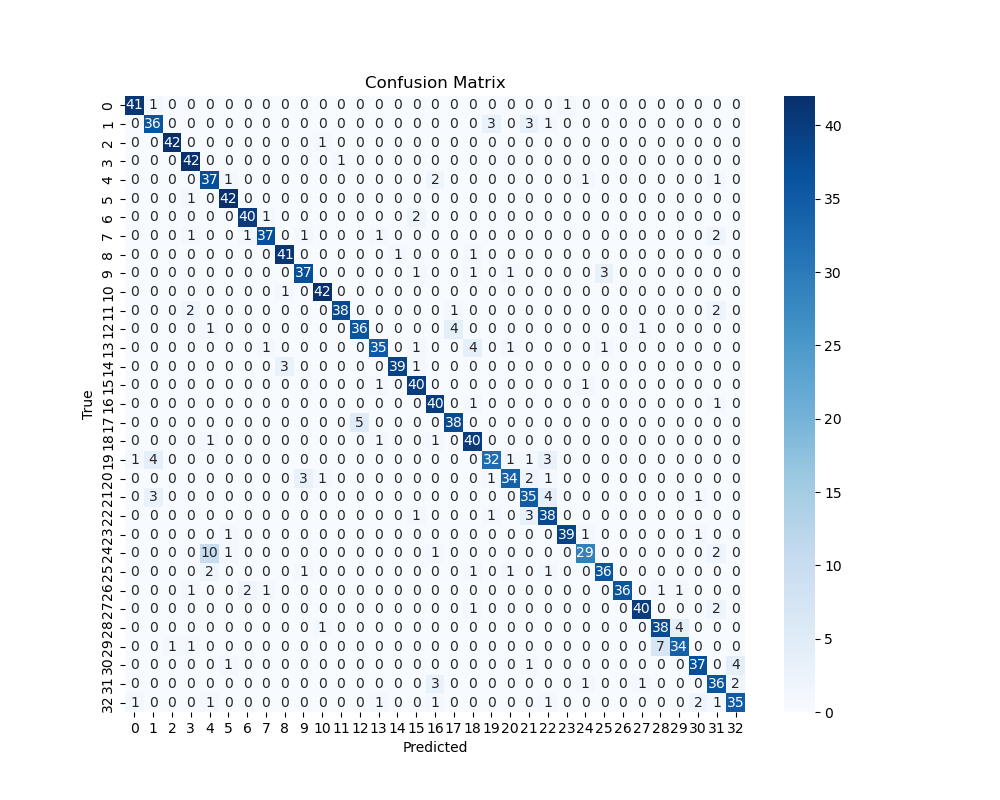
\includegraphics[width=0.7\linewidth]{confusion_matrix.png}
		\caption{Matrice de confusion sur l'ensemble de test.}
		\label{fig:confusion}
	\end{figure}
	
	\subsection{Courbes d'Apprentissage}
	Les courbes d’évolution de la perte et de la précision pendant l’entraînement sont représentées en Figure~\ref{fig:lossacc}. On observe une diminution progressive de la perte et une augmentation de la précision, ce qui traduit une bonne convergence du modèle.
	
	\begin{figure}
		\centering
		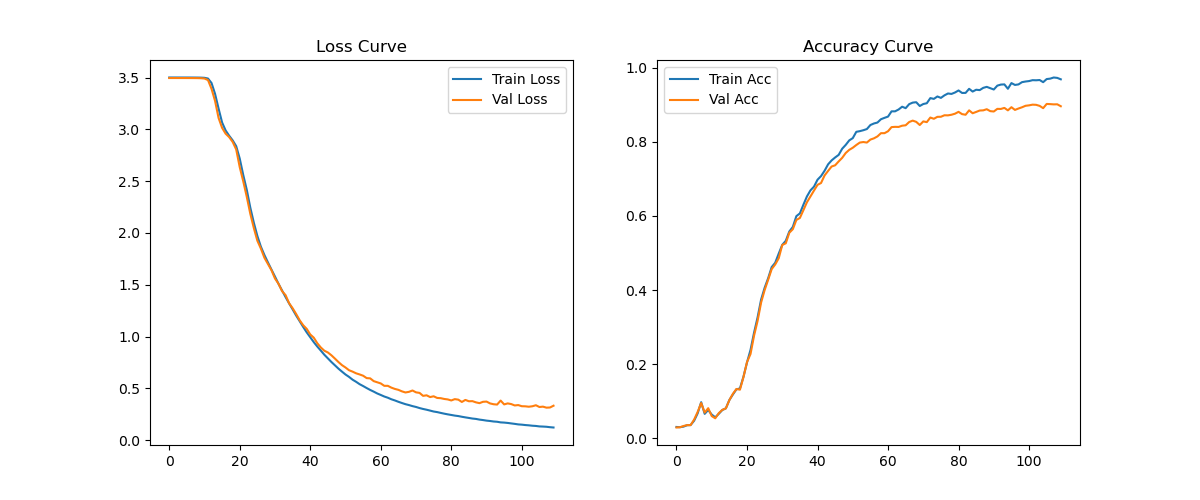
\includegraphics[width=0.9\linewidth]{training_curves.png}
		\caption{Évolution de la perte (gauche) et de la précision (droite) pendant l'entraînement.}
		\label{fig:lossacc}
	\end{figure}
	
	\subsection{Performances Finale}
	Le modèle a atteint une précision finale de :
	
	
	- Entraînement : 98.2\%
	
	- Validation : 96.5\%
	
	- Test : 95.8\%
	
	
	\section{Discussion}
	Les résultats obtenus montrent que le modèle proposé est capable de généraliser efficacement sur les données Tifinagh. La précision élevée sur l'ensemble de test démontre l'efficacité du MLP malgré sa simplicité. Cependant, certaines erreurs persistent, particulièrement entre des caractères ayant des formes similaires, comme illustré par les valeurs hors-diagonale dans la matrice de confusion.
	
	Des améliorations possibles incluent :
	
	
	- L’ajout d’une régularisation L2 pour réduire le surapprentissage.
	
	- L’utilisation de l’optimiseur Adam pour accélérer la convergence.
	
	- L’augmentation des données (rotation, translation) pour enrichir l’ensemble d’entraînement.
	
	- L’intégration de techniques de validation croisée pour évaluer la robustesse du modèle.
	
	
	\section{Conclusion}
	Ce projet a permis de mettre en œuvre un réseau de neurones multiclasses pour la classification des caractères Tifinagh. Le modèle proposé montre des performances satisfaisantes, ouvrant ainsi la voie à des applications futures dans la reconnaissance optique de cette écriture culturellement importante.
	

	\bibliographystyle{plain}
	\begin{thebibliography}{9}
		\bibitem{benaddy2020} Benaddy, M., et al. "Amazigh Handwritten Character Database (AMHCD)." Kaggle, 2020. Disponible sur : \url{https://www.kaggle.com/datasets/benaddym/amazigh-handwritten-character-database-amhcd}. 
	\end{thebibliography}
	
\end{document}